\documentclass[a4paper, 14pt]{article}
\usepackage[margin=1.6cm]{geometry}
\usepackage[utf8]{inputenc}
\usepackage{minted}
\usepackage[russian]{babel}
\usepackage{amsmath}
\usepackage{graphicx}
\usepackage{changepage}
\usepackage{hyperref}
\usepackage{cases}
\pagestyle{empty}

\hypersetup{
	linkbordercolor = {1 1 1}
}

\usepackage[usenames,dvipsnames,svgnames,table]{xcolor}
\usepackage{tikz-timing}[2009/05/15]
\usepackage{multicol}
\usepackage[T2A]{fontenc}
\usepackage{pgfplots}
%\usepackage[left=2.5cm, right=1.5cm, vmargin=2.5cm]{geometry}
\setlength\parindent{0pt} % Удалить отступы из параграфов.

\usepackage{listings}
\usepackage{caption}
\DeclareCaptionFont{white}{\color{white}} % Текст заголовка.
\DeclareCaptionFormat{listing}{\colorbox{gray}{\parbox{\textwidth}{#1#2#3}}}
\captionsetup[lstlisting]{format=listing,labelfont=white,textfont=white}
\renewcommand\labelenumi{\theenumi)}



\begin{document}
\lstset{
	language=java,                 % Выбор языка для подсветки (здесь это java).
	basicstyle=\small\sffamily,    % Размер и начертание шрифта для подсветки кода.
	numbers=left,                  % Где поставить нумерацию строк (слева\справа).
	numberstyle=\tiny,             % Размер шрифта для номеров строк.
	stepnumber=1,                  % Размер шага между двумя номерами строк.
	firstnumber=1,
	numberfirstline=true
	numbersep=5pt,                 % Как далеко отстоят номера строк от подсвечиваемого кода.
	backgroundcolor=\color{white}, % Цвет фона подсветки - используем \usepackage{color}.
	showspaces=false,              % Показывать или нет пробелы специальными отступами.
	showstringspaces=false,        % Показывать или нет пробелы в строках.
	showtabs=false,                % Показывать или нет табуляцию в строках.
	frame=single,                  % Рисовать рамку вокруг кода.
	tabsize=2,                     % Размер табуляции по умолчанию равен 2 пробелам.
	captionpos=t,                  % Позиция заголовка вверху [t] или внизу [b].
	breaklines=true,               % Автоматически переносить строки (да\нет).
	breakatwhitespace=false,       % Переносить строки только если есть пробел.
	escapeinside={\%*}{*)}         % Если нужно добавить комментарии в коде.
}

\begin{titlepage}
	\center

	ФЕДЕРАЛЬНОЕ ГОСУДАРСТВЕННОЕ АВТОНОМНОЕ ОБРАЗОВАТЕЛЬНОЕ УЧРЕЖДЕНИЕ ВЫСШЕГО ОБРАЗОВАНИЯ\linebreak
	«Санкт-Петербургский политехнический университет Петра Великого»\\[2cm]
	\textsc{\Large Институт компьютерных наук и технологий}\\[6.5cm]

	{ \huge \bfseries Курсовая работа	\\
	\Large \mdseries “Реализация Системы Массового Обслуживания”}\\[6.5cm]

	\begin{multicols}{2}
		\begin{flushright} \large

			{Выполнил студент группы: 3530904/00104:}\\[0.5cm]

			{Преподаватель:\\}

		\end{flushright}
		\begin{flushright}

			{Почернин В. С.}\\[0.5cm]


			Смирнов Н. Г.

		\end{flushright}
	\end{multicols}

	\flushright{
		{\today}\\[0.5cm]
	}
	\centering{
		Санкт-Петербург\\
		2022
	}

	\vfill
\end{titlepage}

\large
\tableofcontents
\newpage


\section{Первый этап}


\subsection{Бланк задания с заполненными исходными данными к работе}

\subsubsection{Вариант задания}
ИБ-ИЗ2-ПЗ1-Д10З1-Д10О3-Д2П2-Д2Б2-ОР1-ОД1

\subsubsection{Источники}
\begin{itemize}
	\item ИБ - бесконечный источник.
	\item ИЗ2 - равномерный закон распределения.
\end{itemize}

\subsubsection{Приборы}
\begin{itemize}
	\item ПЗ1 - экспоненциальный закон распределения времени обслуживания.
\end{itemize}

\subsubsection{Описание дисциплин постановки и выбора}
\begin{itemize}
	\item Д10З1 - относительный приоритет на обслуживание - запись в буфер, если есть место по кольцу.
	\item Д1003 - дисциплина отказа - самая старая в буфере.
\end{itemize}

\subsubsection{Дисциплины постановки на обслуживание}
\begin{itemize}
	\item Д2Б2 - принцип выбора заявки из буфера LIFO.
	\item Д2П2 - выбор прибора по кольцу.
\end{itemize}

\subsubsection{Виды отображения результатов работы программной модели}
\begin{itemize}
	\item ОД1 - отображение динамики функционирования модели: календарь событий, буфер и текущее состояние.
	\item ОР1 - отображение результатов: сводная таблица результатов.
\end{itemize}


\subsection{Формализованная схема ВС}
Для освоения функционирования СМО, рассмотрим формализованную схему её работы:
\begin{figure}[!htbp]
	\centering
	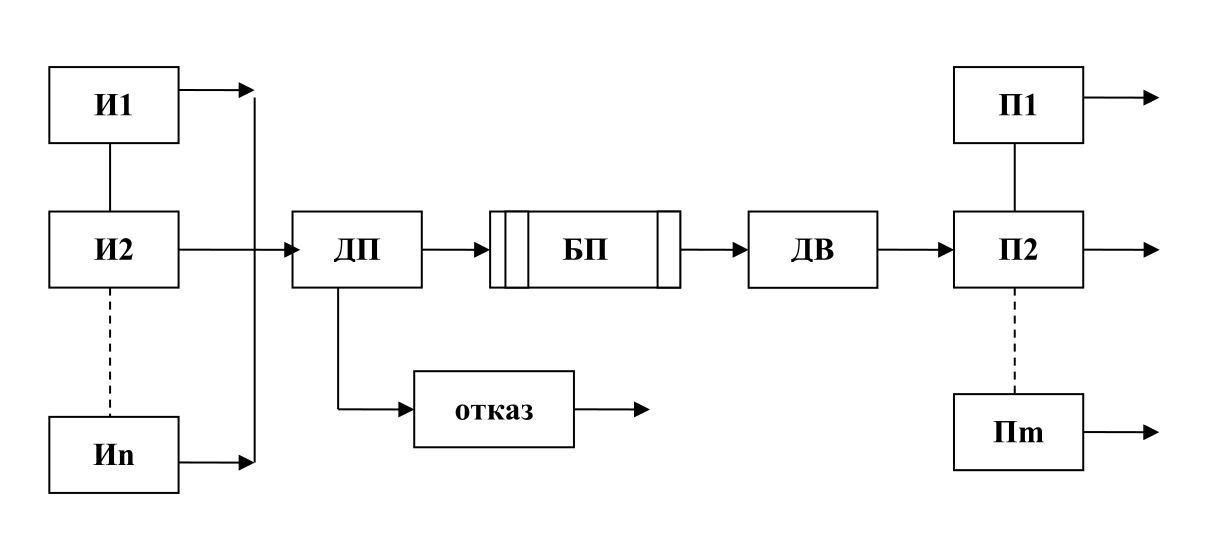
\includegraphics[width=15cm,height=\textheight,keepaspectratio]{smo.png}\\
	\caption{Формализованная схема ВС}
\end{figure}

\begin{itemize}
	\item Иi ($i=1..n$) представляют собой источники заявок, которые генерируют заявки. Все n источников вместе образуют входной поток заявок.
	\item Заявки, сгенерированные в источниках попадают на ДП - диспетчер постановки заявок в очередь. Он организует отказ или выбивание заявки из БП, если в буфере не осталось свободных мест, либо же отправляет заявку на обслуживание или в буферную память в случае отсутствия свободных приборов.
	\item БП - буферная память (место для хранения очереди заявок),  в которой хранятся заявки от различных источников.
	\item ДВ - диспетчер выбора заявок из очереди отправляет заявку из буфера на свободный прибор.
	\item П - приборы, которые обслуживают заявки и создают тем самым выходной поток заявок после обслуживания.
\end{itemize}

На основе этого, мы можем проследить путь заявки, вошедшей в модель системы:
\begin{enumerate}
	\item Постановка заявки в буфер.
	\item Отказ или выбивание (удаление) заявки из переполненного буфера.
	\item Выбор заявки из БП на обслуживание.
	\item Поиск свободного прибора.
	\item Обслуживание заявки прибором.
	\item Выход заявки из СМО.
\end{enumerate}
При этом, вся логика прохождения заявок по системе определяется диспетчерами ДП и ДВ, когда источники и приборы их только генерируют и обслуживают соответственно.


\subsection{Временная диаграмма своего варианта}
Рассмотрим временную диаграмму функционирования системы, на которой покажем
\begin{itemize}
	\item Моменты постановки заявок на приборы.
	\item Заполнение буферной памяти по заданной дисциплине постановки заявки в буфер.
	\item Отказ заявке или выбивание её при отсутствии свободных мест в БП.
	\item Функционирование дисциплины выбора заявок из буфера и дисциплины выбора приборов.
\end{itemize}
Пусть наша система будет состоять из 3 источников (И1, И2, И3), 3 позиций в буфере (Б1, Б2, Б3) и 3 приборов (П1, П2, П3). Получим следующую диаграмму:

\begin{tikztimingtable}
	И1 				& L G L L L L L L L L L L G L L L L L L L L L L L L L L L L L L L\\
	И2 				& L L L G L L L L L L G L L L L G L L L L L L L L L L L L L L L L L\\
	И3 				& L L L L L G L L G L L L L L L L L L L L L L L L L L L L L L L L\\
	П1 				& L 14D{1} 15D{2}\\
	П2 				& L L L 12D{2} L L 13D{1}\\
	П3 				& L L L L L 10D{3} L L L L 11D{2}\\
	Б1 				& L G L L L L L L G L L L L L L G L L G L L L L L L L L L L L L L L L\\
	Б2 				& L L L G L L L L L L G L L L L L L L L L L G L L L L L L L L L L L\\
	Б3 				& L L L L L G L L L L L L G L L L L L L G L L L L L L L L L L L L L\\
	\\
	Постановка      & L G L L G L L G L L G L L G L L G L L G L L L L L L L L L L L L L L L L L\\
	Изъятие         & L G L L G L L G L L L L L L L L L L G L L G L L G L L L L L L L L L L L\\
	\extracode
	\tablerules
	\begin{pgfonlayer}{background}
	\end{pgfonlayer}
\end{tikztimingtable}

\begin{itemize}
	\item Вначале мы видим, как 3 заявки поочереди создаются на источниках с первого по третий и, проходя через буфер (заходя туда по кольцу), моментально оказываются на приборах (куда они также попадают по кольцу).
	\item Затем, опять по правилу кольца, заявки с источников 3, 2 и 1 попадают на буферы 1, 2 и 3, в то время, как первые 3 заявки продолжают обрабатываться приборами, следовательно, у нас происходит заполнение буферной памяти.
	\item Внезапно, источник И2 генерирует еще одну заявку, но в буфере уже заполнены места, поэтому, приходится применять дисциплину отказа - самая старая в буфере. Заявка в буфере Б1 от источника И3, являясь самой старой, выбивается из буфера новоиспеченной заявкой от И2.
	\item Далее, по стечению обстоятельств, все три прибора одновременно заканчивают работу над своими заявками, благодаря чему мы можем увидеть работу дисциплин выбора заявок из буфера и выбора приборов. Так, как мы имеем выбор из буфера LIFO, сначала пойдет заявка с Б1, затем с Б3 и только потом Б2. Приборы же, продолжая выбираться по кольцу, возьмут заявки в порядке П1, П2, П3, так как последним прибором, взявшим заявку был П3.
\end{itemize}

\newpage

\subsection{Ответы на контрольные вопросы}

\begin{enumerate}
	\item Назовите типы источников, опишите принципы их работы, различия между ними.

	      \textbf{Ответ:} Источники бывают двух типов: бесконечные и конечные.

	      Бесконечные источники генерируют заявка, после чего определяют (по определенному закону) интервал для генерации следующей заявки. Заявка попадает в систему в момент генерации и проходит по ней свой индивидуальный путь.

	      В конечных источниках в определенный момент генерируется и отправляется в систему пакет заявок (из конечного числа заявок). Каждая заявка проходит свой индивидуальный путь по системе. Следующий пакет от такого источника генерируется тогда, когда последняя заявка из предыдущего пакета удаляется из системы (в результате обслуживания или отказа). Момент генерации определяется случайным интервалом между пакетами и новый пакет состоит из того же количества заявок.
	\item Можно ли сказать, что бесконечный источник есть частный случай конечного?

	      \textbf{Ответ:} Как мне кажется, мы не можем назвать бесконечный источник частным случаем конечного. Действительно, мы можем считать одну заявку пакетом размера 1, однако случае конечного источника мы имеем четкое условие: "Момент генерации следующего пакета определяется событием, когда последняя заявка этого пакета удаляется из системы". В случае эе бесконечного источника следующая заявка может сгенерироваться в любой момент времени, в том числе тогда, когда предыдущая заявка еще находится в системе.
	\item Опишите два принципа построения моделирующего алгоритма, их преимущества и недостатки.

	      \textbf{Ответ:} Существуют два подхода к построению моделирующего алгоритма ВС: подход Дельта-Т и подход особых событий.

	      Подход Дельта-Т является универсальным методом построения моделирующего алгоритма, в котором состояние объекта проверяется через фиксированный интервал времени. Каждый момент времени $t_i=t_{i-1}+\Delta{t_{i-1}}$ мы получаем приближенные значения характеристик исследуемого объекта. Сам промежуток $\Delta{t}$ должен быть настолько мал, чтобы не пропустить событие в моделирующей системе, которое должно быть учтено при выбранной детальности моделирования. Метод удобен тем, что он является универсальным, однако, есть и недостаток: при его использовании постоянно проверяется состояние объектов моделирования, не изменяющихся при особо малых $\Delta{t}$, что делает метод неэффективным.

	      Подход особых событий мы руководствуемся тем, что интервалы времени, в которых состояние не меняется не представляют для нас интереса. Только значимые (изменяющие состояние) переходы системы имеют для нас значение. Они определяются особыми состояниями или событиями, например:
	      \begin{itemize}
		      \item Поступление заявки в СМО (момент генерации заявки источником).
		      \item Освобождение прибора (готовность прибора взять заявку на обслуживание).
		      \item Окончание процесса моделирование, т. е. момент прекращения генерации заявок источниками.
	      \end{itemize}
	      Достоинством является эффективность данного принципа, из-за чего именно он используется в настоящей работе. К недостаткам же можно отнести сопутствующую сложность отслеживания вышеприведенных событий.
	\item Опишите дисциплины буферизации и постановки заявки на обслуживание, заданные в вашем варианте.

	      \textbf{Ответ:} в моем варианте дисциплинами буферизации являются Д10З1 - запись в буфер, если есть место по кольцу и Д1003 - дисциплина отказа - самая старая в буфере. Дисциплинами постановки заявки на обслуживание являются Д2Б2 - принцип выбора заявки из буфера LIFO и Д2П2 - выбор прибора по кольцу. Рассмотрим каждую из них.

	      \begin{itemize}
		      \item Д1031 - запись в буфер, если есть место по кольцу. При такой дисциплине поиск свободного места в буфере осуществляется, начиная с номера места, следующего за последним занятым. В случае, если указатель, который ищет свободное места его не найдет - начнет действовать дисциплина, организующая отказ или выбивание заявки из БП.
		      \item Д1003 - дисциплина отказа - самая старая в буфере. Эта дисциплина рассматривает только время прихода заявок в систему (момент генерации заявок источником). Заявка, раньше других вставшая в буфер получает отказ, уходит из системы и на её место встает пришедшая заявка.
		      \item Д2Б2 - принцип выбора заявки из буфера LIFO (последним пришел - первым обслужен). В этом лсучае раньше других будет выбрана из буфера та заявка, которая пришла последней.
		      \item Д2П2 - выбор прибора по кольцу. Поиск свободных приборов здесь каждый раз начинается с указателя и заявка встает на обслуживание в первый из найденных приборов.
	      \end{itemize}
	\item Назовите некоторые варианты (комбинации) значений входных параметров, при которых на представленной временной диаграмме могут появиться отказы из БП и будут хорошо проиллюстрированы дисциплины выбора приборов и выбора заявок.

	      \textbf{Ответ:} отказы из БП могут появиться тогда и только тогда, когда любой из источников генерирует заявку в то время, как буфер находится в заполненном состоянии. Например, мы получили 6 заявок от источников, 3 отправились на приборы, 3 в буфер (который после этого заполнился). Генерируется 7-я заявка, которой нет места в буфере, из-за чего применяется дисциплина отказа.

	      Выбор заявок можно явно увидеть, если, например, заполнить по очереди весь буфер и заметить, что забираться заявка будет в обратном порядке. Это покажет нам, что буфер работает как стек, то есть по правилу LIFO.

	      Что касается приборов, мы можем заметить их выбор по кольцу в самом начале, когда они начнут по очереди заполняться заявками. Если же затем приборы одновременно закончат обрабатывать заявки, то новыми заявками они начнут заполняться в том же порядке, поскольку указатель кольца начнет с первого прибора (так как последним прибором был последний прибор в кольце).
\end{enumerate}

\section{Второй этап}

\subsection{Описание}

В рамках второго этапа необходимо разраблтать и отдалить программу, которая смоделирует поведение текущей ВС.

В рамках задания необходимо обеспечить:
\begin{itemize}
	\item \textbf{Относительную точность}: 10\%.
	\item \textbf{Доверительную вероятность}: 0.9.
\end{itemize}
Для этого нужно определить необходимое и достаточное количество заявок, которое должно быть сгенерировано источником (чем больше заявок - тем больше точностью получения выходных характеристик).

Существует \textit{связь} между:
\begin{itemize}
	\item Количеством заявок, прошедших через ВС.
	\item Относительной точностью.
	\item Доверительной вероятностью.
	\item Случайной величиной p(A) (вероятностью события A).
\end{itemize}
\begin{equation} \label{inputs-count}
	N = \frac{t_\alpha^2(1-p)}{p\delta^2} \quad \text{, где}
\end{equation}
\begin{itemize}
	\item $N$ - количество заявок, пропущенных через систему.
	\item $p$ - вероятность отказа заявкам в обслуживании.
	\item $t_\alpha$ = 1.643 для $\alpha = 0.9$.
	\item $\delta = 0.1$ - относительная точность.
\end{itemize}

У нас имеется две неизвестные величины ($N$ и $p$). Мы хотим найти $N$ - значит нужно иметь представление о $p$. Для этого произведем \textbf{пристрелку}.

\subsubsection{Пристрелка}

Алгоритм пристрелки будет следующим:

\begin{enumerate}
	\item Назначим некоторое $N_0 = 100$ и проведем с ним процесс моделирования, получив характеристики (включая $p_0$).
	\item Подставим полученные характеристики в \eqref{inputs-count}, вычислив некоторое $N_1$.
	\item Проведем с ним аналогичный процесс моделирования, получим $p_1$.
	\item Сравним $p_1$ с $p_0$:
	      \begin{enumerate}
		      \item Если $|p_0-p_1| < 0.1p_0$, то $N=100$ удовлетворяет заданной точности результатов.
		      \item Если $|p_0-p_1| \ge 0.1p_0$, то мы продолжаем процесс моделирования с новым $N_2$ и так далее до достижения заданной точности результатов.
	      \end{enumerate}
\end{enumerate}

Этот процесс нахождения необходимого количества заявок нужно реализовать в автоматическом режиме, после чего вывести на экран таблицу результатов, полученных с заданной точностью.

\subsubsection{Отражение работы программной модели}

В текущем задании предусмотрены два вида отражения работы программной модели:
\begin{itemize}
	\item Отображение \textbf{динамики} функционирования модели в \textbf{пошаговом} режиме.
	\item Отображение \textbf{результатов} работы программной модели в \textbf{автоматическом} режиме.
\end{itemize}

\paragraph{Динамика в пошаговом режиме}

Здесь нужно отразить изменение состояние ВС при каждом наступлении особого события.

Фиксация осуществляется пошагово, где \textbf{шаг} - расстояние по времени от одного особого события до ближайшего другого.

В текущем задании необходимо отразить работу программной модели в пошаговом режиме в виде \textbf{календаря событий} (календарь событий, буфер, текущее состояние).

Данная функциональность будет реализована посредством четырех частей:

\begin{itemize}
	\item Кнопки перехода вперед/назад/на конкретный шаг.
	\item Текстовое описание текущего шага.
	\item Таблица календарь событий/текущее состояние:
	      \begin{center}
		      \begin{tabular}{|c|c|c|c|}
			      \hline
			      \multicolumn{2}{|c|}{Календарь событий} & Число заявок & Число отказов   \\
			      \hline
			      Событие                                 & Время        &               & \\
			      \hline
			      И1                                      &              &               & \\
			      \hline
			      ...                                     &              &               & \\
			      \hline
			      Иm                                      &              &               & \\
			      \hline
			      П1                                      &              &               & \\
			      \hline
			      ...                                     &              &               & \\
			      \hline
			      Пk                                      &              &               & \\
			      \hline
			      Конец мод.                              &              &               & \\
			      \hline
		      \end{tabular}
	      \end{center}
	      \begin{itemize}
		      \item Событие - наименование описываемого элемента.
		      \item Время - абсолютное время очередного события (например, время, когда источник сгенерирует заявку или когда прибор обработает заявку).
		      \item Число заявок - число созданных (в случае источника) или обслуженных (в случае прибора) заявок на данный момент.
		      \item Число отказов - количество отказов на данный момент.
	      \end{itemize}
	\item Таблица буфер:
	      \begin{center}
		      \begin{tabular}{|c|c|c|c|}
			      \hline
			      Позиция & Время постановки & Источник & Заявка \\
			      \hline
			      1       &                  &          &        \\
			      \hline
			      ...     &                  &          &        \\
			      \hline
			      N       &                  &          &        \\
			      \hline
		      \end{tabular}
	      \end{center}
\end{itemize}

\paragraph{Результаты в автоматическом режиме}

Для представления результатов моделирования в автоматическом режиме, в процессе работы программной модели для каждой заявки происходит сбор \textbf{статистической информации} для расчета следующих характеристик системы:

\begin{itemize}
	\item Количество заявок сгенерированных каждым источником.
	\item Вероятность отказа в обслуживании заявок каждого источника:
	      $$p=\frac{m}{n}, \quad \text{где}$$
	      \begin{itemize}
		      \item n - общее количество заявок, сгенерированных источником.
		      \item m - количество заявок этого источника, получивших отказ.
	      \end{itemize}
	\item Среднее время пребывания заявки каждого источника в системе:
	      $$T_{\text{преб}} = T_{\text{обсл}} + T_{\text{БП}}, \quad \text{где}$$
	      \begin{itemize}
		      \item $T_{\text{преб}}$ - среднее время пребывания заявки в системе (время ответа на запрос).
		      \item $T_{\text{обсл}}$ - среднее время обслуживания заявки данного источника.
		      \item $T_{\text{БП}}$ - среднее время пребывания заявки в БП или среднее время ожидания заявки каждого источника.
	      \end{itemize}
	\item Дисперсии $T_{\text{обсл}}$ и $T_{\text{БП}}$.
	\item Коэффициенты использования приборов ($\frac{\text{Суммарное время занятости каждого прибора}}{\text{Общее время реализации}}$).
\end{itemize}

Соответственно, после завершение процесса моделирования должны быть получены две таблицы результатов:

\begin{center}
	\begin{tabular}{|c|c|c|c|c|c|c|c|}
		\hline
		\multicolumn{8}{|c|}{Характеристики источников ВС}                                                                                                   \\
		\hline
		№ источника & Количество заявок & $p_\text{отк}$ & $T_\text{преб}$ & $T_\text{БП}$ & $T_\text{обсл}$ & $\text{Д}_\text{БП}$ & $\text{Д}_\text{обсл}$ \\
		\hline
		И1          &                   &                &                 &               &                 &                      &                        \\
		\hline
		И1          &                   &                &                 &               &                 &                      &                        \\
		\hline
		...         &                   &                &                 &               &                 &                      &                        \\
		\hline
		Иm          &                   &                &                 &               &                 &                      &                        \\
		\hline
	\end{tabular}
\end{center}

\begin{center}
	\begin{tabular}{|c|c|}
		\hline
		\multicolumn{2}{|c|}{Характеристики приборов ВС} \\
		\hline
		№ прибора & Коэффициент использования            \\
		\hline
		П1        &                                      \\
		\hline
		П2        &                                      \\
		\hline
		...       &                                      \\
		\hline
		Пk        &                                      \\
		\hline
	\end{tabular}
\end{center}

Отдельно стоит отметить, что \textbf{окончание процесса генерации заявок} (конец моделирования) происходит в момент \textbf{генерации последней заявки}, однако в СМО могут остаться заявки как на приборах, так и в буферной памяти, поэтому процесс \textbf{обслуживания заявок} продолжается до момента \textbf{выхода из системы последней заявки}.

\textbf{Общим временем реализации} называется время, которым заканчивается обслуживание последней заявки (именно его значение используется при расчете коэффициентов использования приборов).

\subsection{Законы распределения}

При моделировании ВС подразумевается использование двух законов распределения:
\begin{itemize}
	\item Равномерный закон распределения времени генерации для бесконечных источников.
	\item Экспоненциальный закон распределения времени обслуживания для приборов.
\end{itemize}
Рассмотрим каждый из них.

\subsubsection{Равномерный закон распределения}

Равномерный закон распределения характеризуется функцией распределения вида:

\begin{equation*}
	F(x) =
	\begin{cases}
		0,               & x < a         \\
		\frac{x-a}{b-a}, & a \le x \le b \\
		1                & x > b
	\end{cases}
\end{equation*}

Построим график распределения при $a = 22$ и $b = 55$:

\begin{tikzpicture}[
		declare function={
				func(\x,\a,\b) =
				(\x < \a) * (0) +
				and(\x >= \a,\x <= \b) * ((\x-\a) / (\b-\a)) +
				(\x>\b) * (1);
			}
	]
	\begin{axis}[
			title = Равномерный закон распределения,
			xlabel = {$x$},
			xmin=0,
			xmax=100,
			ylabel = {$F(x)$},
			minor tick num = 2
		]
		\addplot[
			color=blue,
			domain=0:100,
		]{func(x, 22, 55)};
	\end{axis}
\end{tikzpicture}

Соответственно:
\begin{equation}
	x=F(x)(b-a)+a
\end{equation}

Где $F(x)$ будет случайным числом в диапазоне от 0 до 1.

\subsubsection{Экспоненциальный закон распределения}

Экспоненциальный закон распределения характеризуется функцией распределения вида:
\begin{equation*}
	F(x) = 1 - e^{-\lambda x}
\end{equation*}

Построим график распределения при $\lambda = 3$:

\begin{tikzpicture}
	\begin{axis}[
			title = Экспоненциальный закон распределения,
			xlabel = {$x$},
			xmin=0,
			xmax=100,
			ylabel = {$F(x)$},
			minor tick num = 2
		]
		\addplot[
			color=blue,
			domain=0:100,
		] {1-e^(-0.1*x)};
	\end{axis}
\end{tikzpicture}

Соответственно:
\begin{equation}
	x = -\frac{1}{\lambda}log_e(1-F(x))
\end{equation}
Где F(x) будет случайным числом в диапазоне от 0 до 1.


\subsection{Ответы на контрольные вопросы}

\begin{enumerate}
	\item Какие изменения состояние ВС должны фиксировать программа для текущего задания в пошаговом режиме?

	      \textbf{Ответ:} Мы работаем с методом особых состояний, а значит, что для нас имеют значение только значимые (изменяющие состояние) переходы системы в некоторые моменты времени. Они будут определяться следующими состояниями или событиями:
	      \begin{itemize}
		      \item Поступление заявки в СМО (момент генерации заявки источником).
		      \item Поступление заявки в БП (либо же срабатывание отказа).
		      \item Переход заявки из буфера в свободный прибор.
		      \item Освобождение прибора (и взятие им заявки из буфера, при наличии таковых).
		      \item Окончание процесса моделирования (момент прекращения генерации заявок источниками).
		      \item Выход из системы последней заявки.
	      \end{itemize}
	\item Что должно являться шагом при работе программной модели в режиме динамического отражения результатов?

	      \textbf{Ответ:} При работе программной модели в режиме динамического отражения результатов \textbf{шаг} - это интервал модельного времени от одного особого события до другого ближайшего по времени особого события.
	\item Из чего складывается время пребывания заявки в системе и как рассчитывать среднее время пребывания заявки в системе?.

	      \textbf{Ответ:} Время пребывания заявки в системе рассчитывается по следующей формуле:
	      $$T_{\text{преб}} = T_{\text{обсл}} + T_{\text{БП}}, \quad \text{где}$$
	      \begin{itemize}
		      \item $T_{\text{преб}}$ - среднее время пребывания заявки в системе (время ответа на запрос).
		      \item $T_{\text{обсл}}$ - среднее время обслуживания заявки данного источника.
		      \item $T_{\text{БП}}$ - среднее время пребывания заявки в БП или среднее время ожидания заявки каждого источника.
	      \end{itemize}
	      Чтобы рассчитать именно \textbf{среднее} время - будем для каждого источника суммировать времена заявок и их количество, а затем возьмем среднее арифметическое.
	\item Как рассчитать коэффициент использования приборов $K_{\text{исп}}$?

	      \textbf{Ответ:} $\text{Коэффициент использования приборов} = \frac{\text{Суммарное время занятости каждого прибора}}{\text{Общее время реализации}}$.
	\item В чем разница между окончанием моделирования и общим временем реализации?

	      \textbf{Ответ:}
	      \begin{itemize}
		      \item \textbf{Окончание процесса моделирования} (конец моделирования, окончание процесса генерации заявок) происходит в момент \textbf{генерации последней заявки}, но в этот момент в СМО еще могут оставаться заявки как на приборах, так и в буферной памяти.
		      \item \textbf{Общее время реализации} - это время, которым заканчивается обслуживание последней заявки. То есть момент выхода из системы последней заявки.
	      \end{itemize}
	\item Какие сведения должны быть выведены на экран по истечении времени реализации?.

	      \textbf{Ответ:} После истечения времени реализации, на экран должны быть выведены две таблицы результатов:
	      \begin{itemize}
		      \item Характеристики источников ВС.
		      \item Характеристики приборов ВС.
	      \end{itemize}
\end{enumerate}

\section{Третий этап}

\subsection{Описание}

На третьем этапе нужно привести пример потенциально-существующей ВС (реальной или гипотетической), которая бы полностью соответствовал бы дисциплинам и законам варианта задания.

Стоит учесть, что приводимая система должна быть не просто системой массового обслуживания, а обязательно \textbf{вычислительной} системой - то есть приборами, обслуживающими заявки, должны быть исключительно \textbf{средства вычислительной техники}.

Также нужно иметь достаточно четкое представление о моделируемой системе, чтобы написать количественные значения входных параметров.

В итоге, мы хотим получить выходные характеристики и сравнить их со сформулированными требованиями к результатам работы.

\subsubsection{Определение эффективности ВС}

Определять эффективность нашей ВС будем по следующим выходным характеристикам:

\begin{itemize}
	\item $p_\text{отк}$ - вероятность отказа в обслуживании заявок;
	\item $T_\text{преб}$ - среднее время пребывания заявок в СМО;
	\item $K_\text{исп}$ - коэффициент использования приборов;
\end{itemize}

Задавая желаемые количественные значения этим трём выходным характеристикам, мы формируем требования к работе создаваемой ВС.

\subsubsection{Подход к проектированию модели}

Говоря грубо, мы должны определить, что нужно подать на вход нашей модели, чтобы получить подходящие нам выходные характеристики.

Однако, комбинаций входных значений может оказаться бесконечное множество, поэтому на множество входных значений следует наложить ограничения, исходя из особенности конкретно нашей ВС.

Таким образом, будет спроектирована модель архитектуры системы, которая будет работать по заданным требованиям.

\subsection{Пример ВС, соответствующей модели}

\subsubsection{Непосредственно ВС}

Приведем \textbf{пример потенциально-существующей ВС}, которая бы соответствовала всем законам и дисциплинам нашей модели:


\paragraph{Легенда}

\begin{itemize}
	\item Мы являемся фирмой, выращивающей и подготавливающей для продажи декоративные растения.
	\item Мы выращиваем растения, профессиональные садовники (флористы) всячески их обрабатывают, превращая растения в товар, который мы продаем..
	\item Так как работаем мы с влиятельными клиентами (в основном, наш род деятельности - гос. заказы), нам важен не только заработок, но и наша репутация - мы не можем себе позволить продавать самые старые растения, чтобы побыстрее "слить" их, пока они не завяли, наоборот - чем новее и долговечнее товар мы продадим - тем выгодней для нас (получим больше выгодных сделок).
\end{itemize}

\paragraph{Описание системы}

\begin{center}
	\begin{tabular}{|p{0.2\linewidth} | p{0.3\linewidth}| p{0.5\linewidth}|}
		\hline
		Часть системы      & Описание закона/дисциплины                                                           & Соответствие с реальной ВС                                                                                                                                                                                                                                                                                                                                                       \\
		\hline
		Источники          & Бесконечный источник с равномерным законом распределения времени генерации заявок.   & Источники в нашей системе - это \textbf{грядки}, на которых восходят растения. Мы засаживаем все свободные грядки самыми разными видами семян. Соответственно, время генерации, то есть выращивания равномерно распределено между самым быстрорастущим растением и самым долгорастущим.                                                                                          \\
		\hline
		Приборы            & Экспоненциальный закон распределения времени обслуживания заявок.                    & Приборами у нас являются \textbf{садовники (флористы)}, которые принимают свежевыращеное растения и придают ему товарный вид (обрезают листки, задают форму и т.д.). В зависимости от того, что пришло нашему садовнику (какой-нибудь цветок или целое дерево) - он может обрабатывать его либо очень быстро, либо долго, что и показывает экспоненциальный закон распределения. \\
		\hline
		Буфер              &                                                                                      & Буфером у нас будет \textbf{склад}, где отдельно друг от друга будут храниться растения выращенные, но пока не отправленные на обработку.                                                                                                                                                                                                                                        \\
		\hline
		Постановка в буфер & Запись в буфер, если есть место по кольцу.                                           & Каждое место склада у нас \textbf{равноправно}, соответственно, очередное растение будем ставить на первое свободное место. По кольцу.                                                                                                                                                                                                                                           \\
		\hline
		Отказ в буфере     & Если при постановке в буфер в нем нет мест - из него выбивается самая старая заявка. & Здесь стоит вспомнить, что мы дорожим репутацией и в случае, если выросло новое растение, но его некуда пристроить, оно встанет на место \textbf{самого старого} (уже, возможно, увядающего) растения на складе.                                                                                                                                                                 \\
		\hline
		Выбор из буфера    & Выбор заявки по LIFO(стек).                                                          & Мы хотим, чтобы готовый товар состоял только из самых свежих растений, поэтому в случае, если склад не пуст - мы будем брать \textbf{самое молодое} растение на обработку.                                                                                                                                                                                                       \\
		\hline
		Выбор прибора      & Выбор прибора по кольцу.                                                             & Все флористы у нас также \textbf{равноправны} и нужно их равномерно загрузить, соответственно, будем выбирать первого свободного флориста по кольцу.                                                                                                                                                                                                                             \\
		\hline
	\end{tabular}
\end{center}

\paragraph{Ограничения и требуемые характеристики}

Согласно нашей системе, можно выдвинуть следующие ограничения:

\begin{itemize}
	\item \textbf{Вероятность отказа} должна составлять \textbf{не более 15\%} - мы не хотим, чтобы много растений уходило "в никуда", все-таки, вырастить их - это труд.
	\item \textbf{Коэффициент использования приборов} должен быть \textbf{более 85\%} - все время, что работают садовники (флористы) - это их рабочее время, за которое им платят. Поэтому хотелось бы работать без простоев.
	\item \textbf{Среднее время пребывания заявок в СМО} должно быть \textbf{не более 80 единиц}. Мы считаем, что если растение не превращается в продукт в течение 80 единиц после созревания - оно теряет свою красоту. Эта политика нашей компании дает клиентам гарантию свежести.
\end{itemize}

\begin{center}
	\begin{tabular}{|p{0.5\linewidth} | p{0.5\linewidth}|}
		\hline
		Количество источников (грядок)        & от 4 до 20                                                                                                            \\
		\hline
		Размер буфера (склада)                & от 2 до 15                                                                                                            \\
		\hline
		Количество приборов (садовников)      & от 3 до 15                                                                                                             \\
		\hline
		Скорость работы источников (грядок)   & $a = 10$, $b = 100$                                                                                                   \\
		\hline
		Скорость работы приборов (садовников) & $\lambda = 0.01$ - садовники 1го разряда \par $\lambda = 0.02$ - садовники 2го разряда \par $\lambda = 0.03$ - садовники 3го разряда \\
		\hline
	\end{tabular}
\end{center}

\paragraph{Примечание}

\begin{itemize}
	\item Чем выше класс садовника, тем выше его стоимость.
	\item Время задается в днях.
\end{itemize}

\subsubsection{Ответы на контрольные вопросы}

\begin{enumerate}
	\item Опишите элементы СМО для примера своего варианта ВС по следующей схеме:
	      \begin{itemize}
		      \item Источник - тип и характеристики.
		      \item Прибор - количество и характеристики.
		      \item Буфер - тип и характеристики.
		      \item Заявка - транзакция конкретного размера.
	      \end{itemize}

	      \textbf{Ответ:} указано в таблицах.
	\item Соответствуют ли случайные законы и дисциплины постановки и выбора вашей ВС законами и дисциплинами, указанными в строчке задания вашего варианта?

	      \textbf{Ответ:} да, соответствуют, указано в таблицах.
	\item Значениями каких выходных характеристик определяется качество работы системы?

	      \textbf{Ответ:}
	      Качество работы системы определяется следующими выходными характеристиками:

	      \begin{itemize}
		      \item $p_\text{отк}$ - вероятность отказа в обслуживании заявок;
		      \item $T_\text{преб}$ - среднее время пребывания заявок в СМО;
		      \item $K_\text{исп}$ - коэффициент использования приборов;
	      \end{itemize}
	\item Составьте требования к работе ВС (значения, которые вы хотите получить для выходных характеристик)

	      \textbf{Ответ:} составлено выше.
	\item Напишите ограничения (область изменения) для всех пяти входных параметров исследуемой ВС.

	      \textbf{Ответ:} составлено выше в таблице.
\end{enumerate}

\end{document}